\documentclass[tikz, border=2mm]{article}
\usepackage{karnaugh-map}

\usepackage[utf8]{inputenc}

\usepackage{amsmath}
\usepackage{array}
\newcolumntype{C}{>$c<$}

\title{Tutorato Architettura degli Elaboratori Modulo 1 \\ Lezione 3}
\author{Francesco Pelosin}
\date{4 Novembre 2019}


\begin{document}

\maketitle

\section{Algebra di Boole}

L’aritmetica binaria \`e stata adottata perché i bit sono rappresentabili naturalmente tramite elementi elettronici, codificando lo 0 con uno stato di potenziale elettrico basso e l'1 con uno stato di potenziale elettrico alto.
Il funzionamento dei circuiti elettronici pu\`o essere modellato tramite l’algebra di Boole dove:

\begin{itemize}
    \item Valore logico \texttt{False} $(0)$ $\rightarrow$ livello di potenziale basso.
    \item Valore logico \texttt{True} $(1)$ $\rightarrow$ livello di potenziale alto.
\end{itemize}

\noindent Le operazioni logiche dell'algebra Booleana sono: 
\begin{itemize}
    \item Somma \texttt{OR} $(+)$
    \item Prodotto \texttt{AND} $(\cdot)$
    \item Inversione \texttt{NOT} $(\sim)$
\end{itemize}

\begin{equation*}
    \begin{array}{c c c c c}
    
        \begin{array}{c|c|c}
        A & B & A+B\\
        \hline
        0 & 0 & 0\\
        0 & 1 & 1\\
        1 & 0 & 1\\
        1 & 1 & 1\\
        \end{array}
        &      &
        
        \begin{array}{c|c|c}
        A & B & A\cdot B\\
        \hline
        0 & 0 & 0\\
        0 & 1 & 0\\
        1 & 0 & 0\\
        1 & 1 & 1\\
        \end{array}
        &      &
        
        \begin{array}{c|c}
        A & \sim A\\
        \hline
        0 & 1\\
        1 & 0\\
        \end{array}

    \end{array}
\end{equation*}

\newpage

\noindent Infine ricordiamo le propriet\`a dell'algebra di Bool:
\begin{itemize}
    \item Identità: $$A+0=A$$ $$A\cdot1=A$$
    \item Nullo: $$A+1=1$$ $$A\cdot0=0$$
    \item Idempotente:  $$A+A=A$$  $$A\cdot A=A$$
    \item Inverso:  $$A+(\sim A)=1$$ $$ A\cdot(\sim A)=0$$
    \item Commutativa:  $$A+B=B+A$$  $$A\cdot B=B\cdot A$$
    \item Associativa: $$ A+(B+C)=(A+B)+C$$  $$A\cdot(B\cdot C)=(A\cdot B)\cdot C$$
    \item Distributiva:  $$A\cdot (B+C)=(A\cdot B)+(A\cdot C)$$  $$A+(B\cdot C)=(A+B)\cdot (A+C)$$
    \item DeMorgan:  $$\sim (A+B)=(\sim A)\cdot (\sim B)$$ $$\sim (A\cdot B)=(\sim A)+(\sim B)$$
\end{itemize}

\subsection{Esercizi}
Verificare le seguenti uguaglianze Booleane:
\begin{enumerate}
    \item $A+(B\cdot C)=(A+B)\cdot (A+C)$
    \item $\sim  (A+C\cdot D+A\cdot (\sim  B))=\sim  A\cdot (\sim  C+\sim  D)$
    \item $A\cdot (B+C)+\sim  (A+\sim  C)=A\cdot B+C$
\end{enumerate}

\noindent Semplificare le seguenti espressioni Booleane:
\begin{enumerate}
    \item[4.] $F=A\cdot (B+C)+\sim  B\cdot (A+C)$
    \item[5.] $F=\sim  (\sim  (A+B)\cdot C)$
    \item[6.] $F=\sim  A\cdot B+A\cdot \sim B+\sim  (A+B\cdot C)$
\end{enumerate}

\subsection{Soluzioni}
\begin{enumerate}
    \item Verifichiamo l'uguglianza confrontando le tablelle di verità di $X=A+(B\cdot C)$ e $Y=(A+B)\cdot(A+C)$:
    \begin{equation*}
        \begin{array}{C|C|C||C|C|C|C|C}
        A & B & C & B\cdot C & \overbrace{(A+B\cdot C)}^{\textbf{(X)}} & A+B & A+C & \overbrace{(A+B)\cdot (A+C)}^{\textbf{(Y)}} \\
        \hline
        0 & 0 & 0 & 0 & 0 & 0 & 0 & 0\\
        0 & 0 & 1 & 0 & 0 & 0 & 1 & 0\\
        0 & 1 & 0 & 0 & 0 & 1 & 0 & 0\\
        0 & 1 & 1 & 1 & 1 & 1 & 1 & 1\\
        1 & 0 & 0 & 0 & 1 & 1 & 1 & 1\\
        1 & 0 & 1 & 0 & 1 & 1 & 1 & 1\\
        1 & 1 & 0 & 0 & 1 & 1 & 1 & 1\\
        1 & 1 & 1 & 1 & 1 & 1 & 1 & 1\\
        
        \end{array}
    \end{equation*}
    \\
    Essendo la tabella di verità di $X$ uguale a quella di $Y$ possiamo affermare che l'uguaglianza $X=Y$ \`e vera.
    Verifichiamo ora l'uguaglianza applicando le propriet\`a dell'algebra di Bool:
    \begin{equation*}
    \begin{aligned}
        Y ={} & (A+B)\cdot(A+C) \overset{Distributiva}{=} A\cdot A+A\cdot C+B\cdot A+B\cdot C\overset{Idempotenza}{=} \\
             = &  A+A\cdot C+B\cdot A+B\cdot C \overset{Distributiva}{=} A\cdot(1+C+B)+B\cdot C\overset{Nullo}{=}\\
             = & A\cdot 1+B\cdot C\overset{Identità}{=}A+B\cdot C=X\\
    \end{aligned}
    \end{equation*}
    
    \newpage
    
    \item Verifichiamo l'uguglianza confrontando le tablelle di verità di:
    $$X=\sim (A+C \cdot D+A \cdot ( \sim B))$$
    $$Y= \sim A \cdot ( \sim C+ \sim D)$$
    
    \begin{leftmath}
        \begin{array}{C|C|C|C|C|C|C|C}
        A & B & C & D & C\cdot D & A\cdot(\sim B) & A+C\cdot D+A\cdot(\sim B) & \overbrace{\sim(A+C\cdot D+A\cdot(\sim B))}^{\textbf{(X)}} \\
        \hline
        0&0&0&0&0&0&0&1 \\
        0&0&0&1&0&0&0&1 \\
        0&0&1&0&0&0&0&1 \\
        0&0&1&1&1&0&1&0 \\
        0&1&0&0&0&0&0&1 \\
        0&1&0&1&0&0&0&1 \\
        0&1&1&0&0&0&0&1 \\
        0&1&1&1&1&0&1&0 \\
        1&0&0&0&0&1&1&0 \\
        1&0&0&1&0&1&1&0 \\
        1&0&1&0&0&1&1&0 \\
        1&0&1&1&1&1&1&0 \\
        1&1&0&0&0&0&1&0 \\
        1&1&0&1&0&0&1&0 \\
        1&1&1&0&0&0&1&0 \\
        1&1&1&1&1&0&1&0
        \end{array}
    \end{leftmath}
    \\\\
    \begin{leftmath}    
        \begin{array}{C|C|C|C|C|C|C}
        A & B & C & D & \sim A & \sim C+\sim D & \overbrace{\sim A\cdot(\sim C+\sim D)}^{\textbf{(Y)}} \\
        \hline
        0&0&0&0&1&1&1 \\
        0&0&0&1&1&1&1 \\
        0&0&1&0&1&1&1 \\
        0&0&1&1&1&0&0 \\
        0&1&0&0&1&1&1 \\
        0&1&0&1&1&1&1 \\
        0&1&1&0&1&1&1 \\
        0&1&1&1&1&0&0 \\
        1&0&0&0&0&1&0 \\
        1&0&0&1&0&1&0 \\
        1&0&1&0&0&1&0 \\
        1&0&1&1&0&0&0 \\
        1&1&0&0&0&1&0 \\
        1&1&0&1&0&1&0 \\
        1&1&1&0&0&1&0 \\
        1&1&1&1&0&0&0 \\
        
        \end{array}
    \end{leftmath}

    Essendo la tabella di verità di $X$ uguale a quella di $Y$ possiamo affermare che l'uguaglianza $X=Y$ \`e vera.
    Verifichiamo ora l'uguaglianza applicando le proprietà dell'algebra di Bool:
    \begin{equation*}
    \begin{aligned}
        X ={} & \sim(A+C\cdot D+A\cdot(\sim B)) \overset{Distributiva}{=} \sim(A\cdot(1+\sim B)+C\cdot D) \overset{Nullo}{=} \\
             = &  \sim(A\cdot 1 + C\cdot D) \overset{Identità}{=}\sim(A+C\cdot D) \overset{DeMorgan}{=} \sim A\cdot\sim(C\cdot D)\overset{DeMorgan}{=}\\
             = & \sim A\cdot(\sim C+\sim D)\overset{ }{=}Y\\
    \end{aligned} 
    \end{equation*}
    
    \item Verifichiamo l'uguglianza confrontando le tablelle di verità di:
    $$X=A\cdot (B+C)+\sim (A+\sim C)$$ 
    $$Y=A\cdot B+C$$
    \begin{leftmath}
        \begin{array}{C|C|C|C|C|C|C|C}
        A & B & C & B+C & A\cdot(B+C) & A+\sim C & \sim(A+\sim C) & \overbrace{A\cdot(B+C)+\sim(A+\sim C)}^{\textbf{(X)}} \\
        \hline
        0 & 0 & 0 & 0 & 0 & 1 & 0 & 0\\
        0 & 0 & 1 & 1 & 0 & 0 & 1 & 1\\
        0 & 1 & 0 & 1 & 0 & 1 & 0 & 0\\
        0 & 1 & 1 & 1 & 0 & 0 & 1 & 1\\
        1 & 0 & 0 & 0 & 0 & 1 & 0 & 0\\
        1 & 0 & 1 & 1 & 1 & 1 & 0 & 1\\
        1 & 1 & 0 & 1 & 1 & 1 & 0 & 1\\
        1 & 1 & 1 & 1 & 1 & 1 & 0 & 1\\
        
        \end{array}
    \end{leftmath}
    \\\\
    \begin{leftmath}
        \begin{array}{C|C|C|C|C}
        A & B & C & A\cdot B & \overbrace{A\cdot B+C}^{\textbf{(Y)}} \\
        \hline
        0 & 0 & 0 & 0 & 0\\
        0 & 0 & 1 & 0 & 1\\
        0 & 1 & 0 & 0 & 0\\
        0 & 1 & 1 & 0 & 1\\
        1 & 0 & 0 & 0 & 0\\
        1 & 0 & 1 & 0 & 1\\
        1 & 1 & 0 & 0 & 1\\
        1 & 1 & 1 & 1 & 1\\
        
        \end{array}
    \end{leftmath}
    
    Essendo la tabella di verità di $X$ uguale a quella di $Y$ possiamo affermare che l'uguaglianza $X=Y$ è vera.
    Verifichiamo ora l'uguaglianza applicando le proprietà dell'algebra di Bool:
    \begin{equation*}
    \begin{aligned}
        X ={} & A\cdot(B+C)+\sim(A+\sim C) \overset{Distributiva}{=} A \cdot B+A\cdot C+\sim(A+\sim C)\overset{DeMorgan}{=} \\
             = &  A\cdot B+A\cdot C+\sim A\cdot\sim\sim C \overset{}{=}A\cdot B+A\cdot C+\sim A\cdot C\overset{Distributiva}{=}\\
             = & A\cdot B+C\cdot(A+\sim A) \overset{Inverso}{=}A\cdot B+C\cdot 1\overset{Identità}{=}A\cdot B+C=Y\\
    \end{aligned} 
    \end{equation*}
    \newpage
    \item Seplifichiamo $F=A\cdot (B+C)+ \sim B\cdot (A+C)$ usando le proprietà dell'algebra di Bool:\\\\
    \begin{leftmath}
    \begin{aligned}
        F ={} & A\cdot(B+C)+\sim B\cdot(A+C) \overset{Distributiva}{=} \\
             = & A\cdot B+A\cdot C+\sim B\cdot A+\sim B\cdot C \overset{Distributiva}{=} \\
             = & A\cdot(B+\sim B)+A\cdot C+ \sim B\cdot C\overset{Inverso}{=}\\
             = & A\cdot 1+A\cdot C+ \sim B\cdot C\overset{Distributiva}{=} \\
             = & A\cdot(1+C)+\sim B\cdot C\overset{Nullo}{=}\\
             = & A+\sim B\cdot C\\
    \end{aligned} 
    \end{leftmath}
    \\
    \item Seplifichiamo $F=\sim (\sim (A+B)\cdot C)$ usando le propriet\`a dell'algebra di Bool:\\\\
    \begin{leftmath}
    \begin{aligned}
        F ={} & \sim(\sim(A+B)\cdot C) \overset{DeMorgan}{=}\\
              = &\sim(\sim A\cdot \sim B\cdot C) \overset{Distributiva}{=}\\
              = &\sim\sim A+\sim\sim B+\sim C\overset{Distributiva}{=}\\
              = & A+B+\sim C\\
    \end{aligned} 
    \end{leftmath}
    \\
    \item Seplifichiamo $F=\sim A\cdot B+A\cdot \sim B+\sim(A+B\cdot C)$ usando le proprietà dell'algebra di Bool:\\\\
    \begin{leftmath}
    \begin{aligned}
        F ={} & \sim A\cdot B+A\cdot\sim B+\sim(A+B\cdot C) \overset{DeMorgan}{=}\\
        = & \sim A\cdot B+A\cdot\sim B+\sim A\cdot \sim(B\cdot C) \overset{DeMorgan}{=} \\
        = & \sim A\cdot B+A\cdot\sim B+\sim A\cdot(\sim B+\sim C)\overset{Distributiva}{=}\\
        = & \sim A\cdot B+A\cdot\sim B+\sim A\cdot\sim B+\sim A\cdot\sim C\overset{Distributiva}{=}\\
        = & A\cdot\sim B+\sim A\cdot(B+\sim B+\sim C)\overset{Inverso}{=}\\
        = & A\cdot\sim B+\sim A\cdot(1+\sim C)\overset{Nullo}{=}\\
        = & A\cdot\sim B+\sim A\cdot1\overset{Identità}{=}\\
        = & A\cdot\sim B+\sim A\overset{Distributiva}{=}\\
        = & (A+\sim A)\cdot(\sim B+\sim A)\overset{Inverso}{=}\\
        = & \sim B+\sim A
    \end{aligned} 
    \end{leftmath}

\end{enumerate}


\newpage



\section{Forme canoniche e Minimizzazione}
Ogni funzione logica pu\`o essere rappresentata come tabella di verità o come equazione logica. \`E possibile ricavare quest'ultima a partire dalla tabella di verità tramite l'uso degli operatori \texttt{AND}, \texttt{OR} e \texttt{NOT}.
Un'equazione logica può essere espressa nei seguenti due modi:
\begin{itemize}
    \item Somma di prodotti: per ogni entry uguale ad 1 dell'output della tabella di verità generiamo un prodotto (mintermine) degli input, dove gli input uguali a 0 appaiono negati. Infine sommiamo tutti i prodotti ottenuti.
    \item Prodotto di somme: per ogni entry uguale ad 0 dell’ouput della tabella di verità generiamo una somma (maxtermine) degli input, dove gli input uguali a 1 appaiono negati. Infine moltiplichiamo tutti le somme ottenute.
\end{itemize}
\subsection{Mappe di Karnaugh}
Per minimizzare a mano funzioni di poche variabili, si possono rappresentare le tabelle di verità con le mappe di Karnaugh in cui:
\begin{itemize}
    \item Ogni quadrato (cella) della mappa individua una combinazione di variabili in input.
    \item Il valore contenuto in una cella corrisponde al valore in output per quella particolare combinazione di variabili di input.
    \item Le combinazioni delle variabili in input che etichettano i due assi delle mappe differiscono di un singolo bit tra combinazioni consecutive.
\end{itemize}
Infine, raggruppando i valori 1 delle mappe di Karnaugh è possibile individuare facilmente insiemi di variabili DON'T CARE. Ricordiamo che i gruppi devono essere composti da $2^i \forall  i \geq 0$ valori uguali uguali ad 1.

\subsection{Esercizi}

Per ogni esercizio definire la tabella delle verità della funzione logica, riportare la forma canonica in somme di prodotti e prodotti di somme e minimizzare attraverso le Mappe di Karnaugh.

\begin{enumerate}
    \item Si vuole costruire un circuito combinatorio con le seguenti caratteristiche:
    \begin{itemize}
        \item Tre input $A,B,C$ e un output $Y$.
        \item Funzione di output così definita: $Y=A \iff C=0, Y=B \iff C=1$.
    \end{itemize}
    
    \item Si vuole costruire un circuito combinatorio con le seguenti caratteristiche:
    \begin{itemize}
        \item Quattro input $A,B,C,D$ e un output $Y$.
        \item Dato $N=ABCD$ numero binario a quattro cifre, definiamo $Y$ come segue: $Y=1  \iff N$ contiene un numero di 1 maggiore o uguale a 2, 0 altrimenti.
    \end{itemize}

    \newpage
    \item Si vuole costruire un circuito combinatorio con le seguenti caratteristiche:
    \begin{itemize}
        \item Quattro input $A,B,C,D$ e un output $Y$.
        \item Dato $N=ABCD$ numero binario a quattro cifre espresso in complemento a due, definiamo $Y$ come segue: $Y=1  \iff N\leq-2$, 0 altrimenti.
    \end{itemize}
    
    \item Rappresentare le precedenti funzioni logiche con un multiplexer.
\end{enumerate}

\subsection{Soluzioni}

\begin{enumerate}

\item Cominciamo scrivendo la tabella di verità della funzione:\\
    \begin{equation*}
        \begin{array}{C|C|C|C}
        A & B & C & Y \\
        \hline
        0 & 0 & 0 & 0\\
        0 & 0 & 1 & 0\\
        0 & 1 & 0 & 0\\
        0 & 1 & 1 & 1\\
        1 & 0 & 0 & 1\\
        1 & 0 & 1 & 0\\
        1 & 1 & 0 & 1\\
        1 & 1 & 1 & 1\\
        
        \end{array}
    \end{equation*}
\\Per prima cosa esprimiamo l'equazione logica associata alla tabella di verità nelle due forme canoniche (somma di prodotti e prodotto di somme):

$$Y_{SP}=\sim A\cdot B\cdot C+A\cdot\sim B\cdot\sim C+A\cdot B\cdot\sim C+A\cdot B\cdot C$$
$$Y_{PS}=(A+B+C)\cdot(A+B+\sim C)\cdot(A+\sim B+C)\cdot(\sim A+B+\sim C)$$

Procediamo ora a minimizzare le due funzioni tramite mappe di Karnaugh:
\begin{center}
\begin{karnaugh-map}[4][2][1][$BC$][$A$]
    \manualterms{0,0,0,1,1,0,1,1}
    \implicant{3}{7}
    \implicantedge{4}{4}{6}{6}

\end{karnaugh-map}
\end{center}
Osservando i raggruppamenti possiamo minimizzare la funzione come segue:
\begin{itemize}
    \item $Y_{SP}=A\cdot\sim C+B\cdot C$
\end{itemize}
\begin{center}
\begin{karnaugh-map}[4][2][1][$BC$][$A$]
    \manualterms{0,0,0,1,1,0,1,1}
    \implicant{1}{5}
    \implicantedge{0}{0}{2}{2}

\end{karnaugh-map}
\end{center}
Osservando i raggruppamenti possiamo minimizzare la funzione come segue:
\begin{itemize}
    \item $Y_{PS}=(A+C)\cdot(B+\sim C)$
\end{itemize}
Si lascia agli studenti come esercizio il compito di disegnare i circuiti corrispondenti.


\item Cominciamo scrivendo la tabella di verità della funzione:\\
    \begin{equation*}
        \begin{array}{C|C|C|C|C}
        A & B & C & D & Y \\
        \hline
        0 & 0 & 0 & 0 & 0\\
        0 & 0 & 0 & 1 & 0\\
        0 & 0 & 1 & 0 & 0\\
        0 & 0 & 1 & 1 & 1\\
        0 & 1 & 0 & 0 & 0\\
        0 & 1 & 0 & 1 & 1\\
        0 & 1 & 1 & 0 & 1\\
        0 & 1 & 1 & 1 & 1\\
        1 & 0 & 0 & 0 & 0\\
        1 & 0 & 0 & 1 & 1\\
        1 & 0 & 1 & 0 & 1\\
        1 & 0 & 1 & 1 & 1\\
        1 & 1 & 0 & 0 & 1\\
        1 & 1 & 0 & 1 & 1\\
        1 & 1 & 1 & 0 & 1\\
        1 & 1 & 1 & 1 & 1\\
        
        
        \end{array}
    \end{equation*}
\\Per prima cosa esprimiamo l'equazione logica associata alla tabella di verità nelle due forme canoniche (somma di prodotti e prodotto di somme):


    \begin{leftmath}
    \begin{aligned}
        Y_{SP}={} & \sim A\cdot \sim B\cdot C\cdot D+\sim A\cdot B\cdot \sim C\cdot D+\sim A\cdot B\cdot C\cdot \sim D+\\
                + & \sim A\cdot B\cdot C\cdot D+A\cdot \sim B\cdot \sim C\cdot D+A\cdot \sim B\cdot C\cdot \sim D+\\
                + & A\cdot \sim B\cdot C\cdot D+A\cdot B\cdot \sim C\cdot \sim D+A\cdot B\cdot \sim C\cdot D+\\
                + & A\cdot B\cdot C\cdot \sim D+A\cdot B\cdot C\cdot D
    \end{aligned}
    \end{leftmath}

    \begin{leftmath}
    \begin{aligned}
        Y_{PS}={} & (A+B+C+D)\cdot(A+B+C+\sim D)\cdot(A+B+\sim C+D)\cdot\\
                \cdot & (A+\sim B+C+D)\cdot(\sim A+B+C+D)\\

    \end{aligned}
    \end{leftmath}

Procediamo ora a minimizzare le due funzioni tramite mappe di Karnaugh:
\begin{center}
\begin{karnaugh-map}[4][4][1][$CD$][$AB$]
    \manualterms{0,0,0,1,0,1,1,1,0,1,1,1,1,1,1,1}
    \implicant{3}{11}
    \implicant{12}{14}
    \implicant{5}{15}
    \implicant{7}{14}
    \implicant{13}{11}
    \implicant{15}{10}
    
\end{karnaugh-map}
\end{center}
Osservando i raggruppamenti possiamo minimizzare la funzione come segue:
\begin{itemize}
    \item $Y_{SP}=C\cdot D+A\cdot B+B\cdot D+A\cdot D+B\cdot C+A\cdot C$
\end{itemize}
\begin{center}
\begin{karnaugh-map}[4][4][1][$CD$][$AB$]
    \manualterms{0,0,0,1,0,1,1,1,0,1,1,1,1,1,1,1}
    \implicant{0}{1}
    \implicant{0}{4}
    \implicantedge{0}{0}{2}{2}
    \implicantedge{0}{0}{8}{8}
    
\end{karnaugh-map}
\end{center}
Osservando i raggruppamenti possiamo minimizzare la funzione come segue:
\begin{itemize}
    \item $Y_{PS}=(A+B+C)\cdot(A+C+D)\cdot(A+B+D)\cdot(B+C+D)$
\end{itemize}
Si lascia agli studenti come esercizio il compito di disegnare i circuiti corrispondenti.
 

\item Cominciamo scrivendo la tabella di verità della funzione:\\
    \begin{equation*}
        \begin{array}{C|C|C|C|C}
        A & B & C & D & Y \\
        \hline
        0 & 0 & 0 & 0 & 0\\
        0 & 0 & 0 & 1 & 0\\
        0 & 0 & 1 & 0 & 0\\
        0 & 0 & 1 & 1 & 0\\
        0 & 1 & 0 & 0 & 0\\
        0 & 1 & 0 & 1 & 0\\
        0 & 1 & 1 & 0 & 0\\
        0 & 1 & 1 & 1 & 0\\
        1 & 0 & 0 & 0 & 1\\
        1 & 0 & 0 & 1 & 1\\
        1 & 0 & 1 & 0 & 1\\
        1 & 0 & 1 & 1 & 1\\
        1 & 1 & 0 & 0 & 1\\
        1 & 1 & 0 & 1 & 1\\
        1 & 1 & 1 & 0 & 1\\
        1 & 1 & 1 & 1 & 0\\
        
        
        \end{array}
    \end{equation*}
\\Per prima cosa esprimiamo l'equazione logica associata alla tabella di verità nelle due forme canoniche (somma di prodotti e prodotto di somme):


    \begin{leftmath}
    \begin{aligned}
        Y_{SP}={} & A\cdot \sim B\cdot \sim C\cdot \sim D+A\cdot \sim B\cdot \sim C\cdot D+A\cdot \sim B\cdot C\cdot \sim D+\\
                + & A\cdot \sim B\cdot C\cdot D+A\cdot B\cdot \sim C\cdot \sim D+A\cdot B\cdot \sim C\cdot D+\\
                + & A\cdot B\cdot C\cdot \sim D\\
    \end{aligned}
    \end{leftmath}

    \begin{leftmath}
    \begin{aligned}
        Y_{PS}={} & (A+B+C+D)\cdot(A+B+C+\sim D)\cdot(A+B+\sim C+D)\cdot\\
                \cdot & (A+B+\sim C+\sim D)\cdot(A+\sim B+C+D)\cdot(A+\sim B+C+\sim D)\\
                \cdot & (A+\sim B+\sim C+D)\cdot(A+\sim B+\sim C+\sim D)\cdot\\
                \cdot & (\sim A+\sim B+\sim C+\sim D)\\
    \end{aligned}
    \end{leftmath}

Procediamo ora a minimizzare le due funzioni tramite mappe di Karnaugh:
\begin{center}
\begin{karnaugh-map}[4][4][1][$CD$][$AB$]
    \manualterms{0,0,0,0,0,0,0,0,1,1,1,1,1,1,1,0}
    \implicant{8}{10}
    \implicant{12}{9}
    \implicantedge{12}{8}{14}{10}
    
\end{karnaugh-map}
\end{center}
Osservando i raggruppamenti possiamo minimizzare la funzione come segue:
\begin{itemize}
    \item $Y_{SP}=A\cdot\sim B+A\cdot\sim C+A\cdot\sim D$
\end{itemize}
\begin{center}
\begin{karnaugh-map}[4][4][1][$CD$][$AB$]
    \manualterms{0,0,0,0,0,0,0,0,1,1,1,1,1,1,1,0}
    \implicant{0}{6}
    \implicant{7}{15}

    
\end{karnaugh-map}
\end{center}
Osservando i raggruppamenti possiamo minimizzare la funzione come segue:
\begin{itemize}
    \item $Y_{PS}=A\cdot(\sim B+\sim C+\sim D)$
\end{itemize}
Si lascia agli studenti come esercizio il compito di disegnare i circuiti corrispondenti.

\newpage

\item Per rappresentare la funzione logica del primo esercizio dobbiamo utilizzare un multiplexer 8:1:
\begin{center} 
    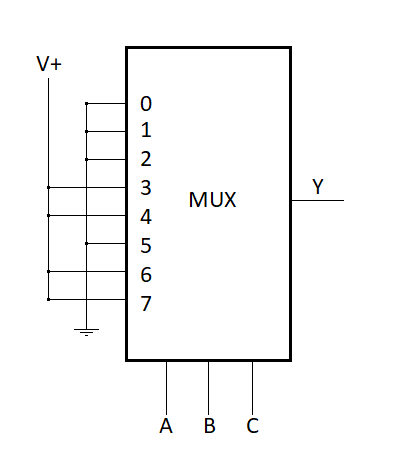
\includegraphics{mux1.png}
\end{center}
Per rappresentare la funzione logica del secondo esercizio dobbiamo utilizzare un multiplexer 16:1:
\begin{center} 
    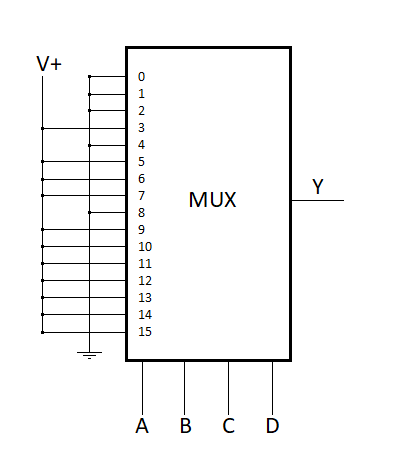
\includegraphics{mux2.png}
\end{center}
Per rappresentare la funzione logica del terzo esercizio dobbiamo utilizzare un multiplexer 16:1:
\begin{center} 
    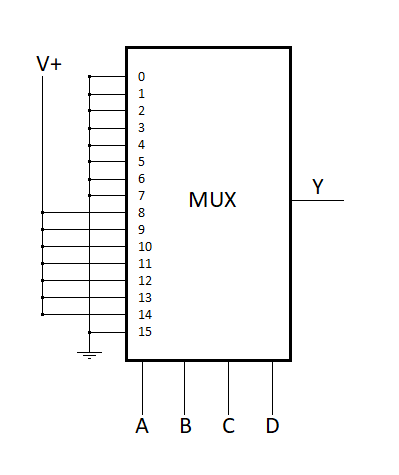
\includegraphics{mux3.png}
\end{center}
In generale, gli ingressi del multiplexer sono i valori della funzione da rappresentare. Ogni ingresso del multiplexer viene selezionato dalla corrispondente combinazione delle variabili di input della funzione, che diventano quindi i segnali di controllo del multiplexer. Ad esempio la linea 5 del terzo multiplexer viene selezionata da: A=0, B=1, C=0, D=1 (valori di ingresso della funzione logica) a cui deve corrispondere Y=0 (valore di uscita nella corrispettiva tabella di verità). Di conseguenza l'ingresso 5 del multiplexer deve essere collegato al valore fisico corrispondente allo 0 (massa). \\

\end{enumerate}

\end{document}
